\chapter{Nuclear transfer reactions}
\label{chapt:reactions}
In terms of nuclear physics, a nuclear reaction occurs when two atomic nuclei collide and transform to produce new nuclei different from the reactants.  Use of a particle accelerator is needed in order for the colliding particles to have sufficient kinetic energy to overcome the Coulomb repulsion due to the nuclear charge.  A special class of nuclear reactions called ``transfer reactions'' involve the transfer of a small number of nucleons between the reactants during the process of the reaction.  This chapter discusses the utility of studying such nuclear reactions and how they provides a powerful analytic tool for understanding  nuclei.  Transfer reactions are one of several methods that allow the study of the position of excited states in a nucleus.  Other methods include $\beta$-decay $\gamma$-decay studies.  What makes transfer reaction studies unique is the way in which they provide information on the quantum number associated with the spin and parity of nuclear energy levels.  In addition, transfer reactions provide information on the single particle structure of a nucleus.

\section{Direct Reactions}
In the most basic form of a direct reaction, an incident beam particle has a single collision with a target nucleus, interacting with a single degree of freedom in the target nucleus.  Direct transfer reactions are characterized by short interaction time $t\sim2r_0/v_1$ where $r_0$ is the radius of the target nucleus and $v_1$ is the velocity of the incident ion.  The amount of energy transferred in these reactions is small compared to the incident beam energy; thus these reactions are sometimes referred to as being  ``quasi-elastic'' to differentiate them from deep-inelastic nuclear reactions. 

\begin{figure}%
\centering
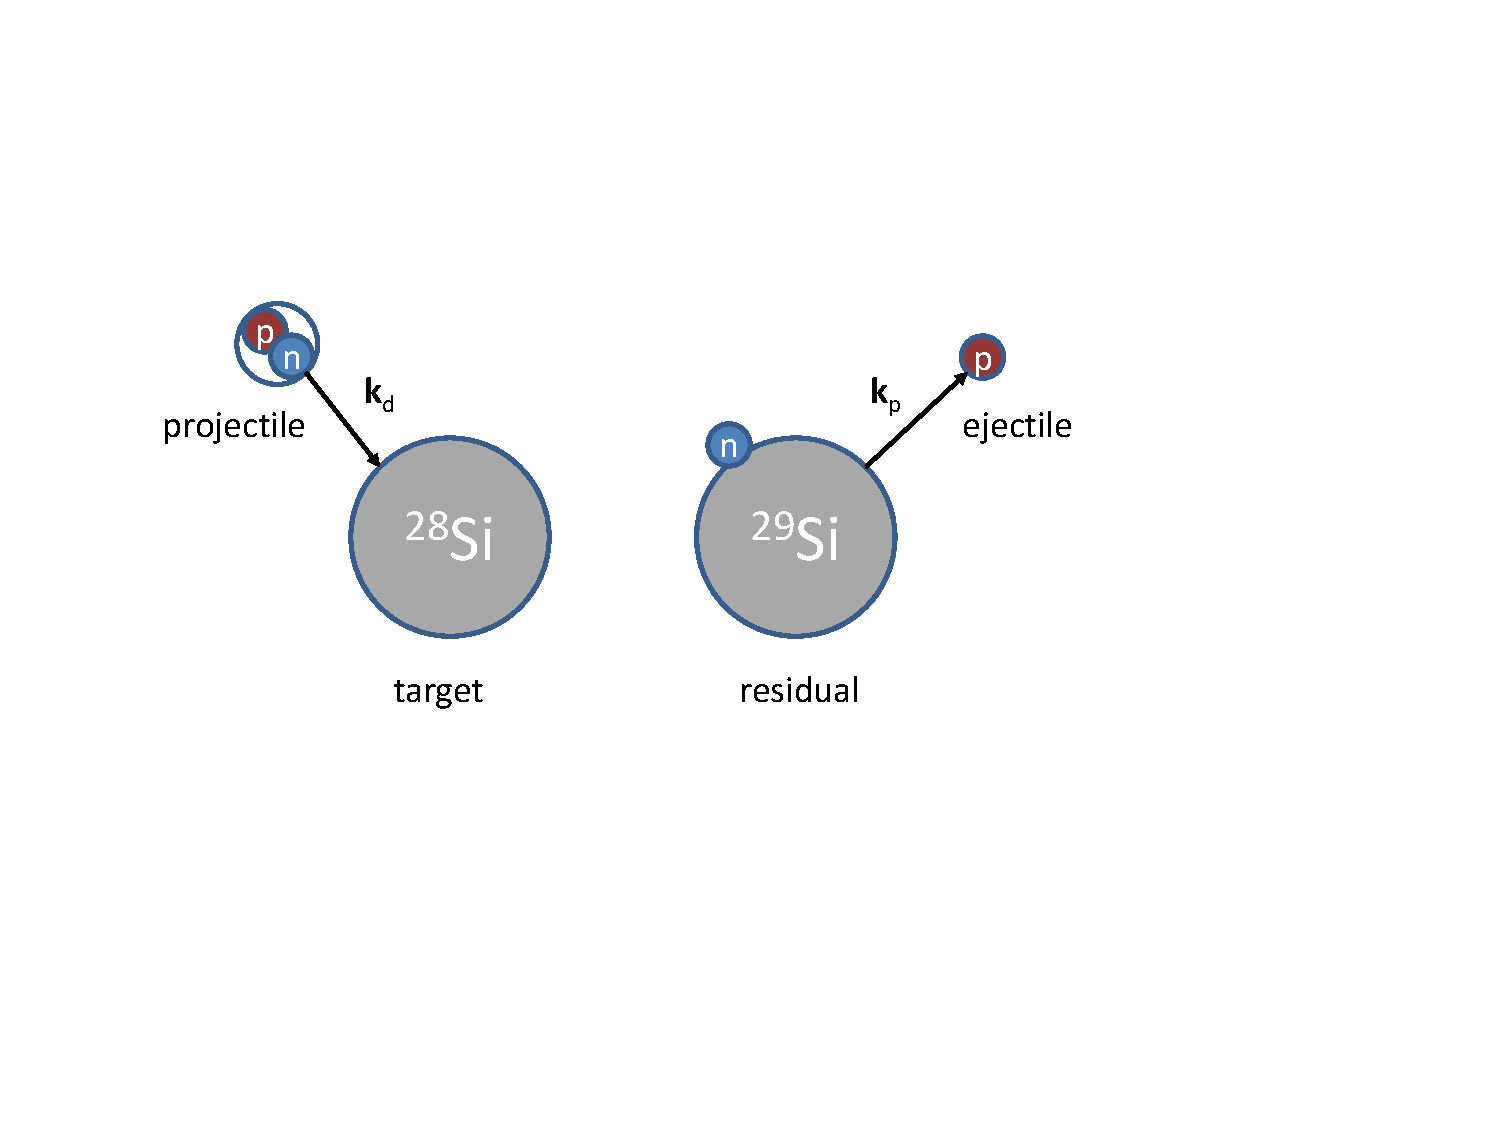
\includegraphics[width=0.75\columnwidth,height=0.33\textheight,keepaspectratio]{dp_schem2}%
\caption[Schematic illustration of the ($d$,$p$) reaction]{Schematic illustration of the ($d$,$p$) reaction.  The  deuteron has an incident momentum of $k_d$. After colliding with the $^{28}$Si target nucleus, the neutron is stripped from the beam particle and the proton has an outgoing momentum of $k_p$.}%
\label{dp_fig}%
\end{figure}

\subsection{Notation}
In the prototypical example, a stationary target is bombarded by an accelerated beam of particles and a detector measures the scattered particles.  The reaction may be written as
\begin{equation}
A+a\rightarrow B+b
\label{basic_reaction}
\end{equation}
where $A$ is the heavy ion reactant; $a$ is the light ion reactant; $B$ is the heavy ion recoil; and $b$ is the light ion recoil.  In this notation, the reaction can be written in a more compact form as $A$($a$,$b$)$B$ with ($a$,$b$) identifying the type of reaction.   

This notation convention was developed during a time with the reactions being studied typically involved a light ion beam and a heavy ``ion'' target---here the term ion is used loosely, as the target are not typically ionized.  To make consistent use of this notation, the first reactant listed is defined as the target nucleus and the second reactant is defined as the beam particle or projectile.  Therefore, under this convention, a reaction in which the heavy reactant is accelerated (``inverse kinematics'') would be written as $a$($A$,$b$)$B$, even though the reaction would still be referred to as an ``($a$,$b$)'' reaction.  Similarly, the light ion ejectile $b$ is traditionally the detected particle, or the particle of interest.  Adopting the notation, a reaction in which the heavy recoil is the particle of interest or a measurement in which the heavy ion is detected can be written as $A$($a$,$B$)$b$. 

In elastic scattering, the incoming particle $a$ and the outgoing particle $b$ are the same, leaving the ion species of the target nucleus unchanged.  In a transfer reaction,  $a$ and $b$ are different from each other.  The form of this difference divides transfer reactions into three different classes, given names from the perspective of the light ion projectile.  For example, in a ``stripping'' reaction, nucleons are stripped from the incident projectiles by the target nucleus.  Examples of stripping reactions include ($d$,$p$) and ($^3$He,$d$) which are neutron and proton stripping reactions, respectively.  These reactions add nucleons to the target nucleus.  The inverse of this process is referred to as a ``pick-up'' reaction, where the incident projectile picks-up nucleons from the target.  For example ($d$,$^3$He) and ($t$,$\alpha$) are proton pick-up reactions.

In a typical nucleon transfer reaction, a heavy target is bombarded by an accelerated beam of stable light nuclei.  A classic example of such a reaction is a deuteron beam striking a stable $^{28}$Si target to produce $^{29}$Si~\cite{Mermaz_1971}, illustrated in Fig.~\ref{dp_fig}.  In such an experiment, the ejected proton is detected in order to study the properties of $^{29}$Si.  Traditionally, the ejected light ion is detected with silicon detectors through a range of fixed laboratory angles---other detectors may also be used, such as photographic plates, gas counters, \textit{etc.}  Charge collection in the detectors determines the ejected particle's energy and the position of the detector determines the laboratory angle.  Detectors can be segmented or position-sensitive for enhanced angular resolution.
 
\subsection{Single-particle States}
What makes direct nuclear reactions unique is the wealth of information they provide and the relative ease with which they provide it.  In a traditional experiment, involving an isotopically pure beam and a target which is either isotopically pure or of a known composition, there is little question as to the source of the measured results.  In turn, this makes particle identification nearly unnecessary, eliminating the need for additional detectors and electronics.

Single particle states around closed-shell nuclei serve as a benchmark for testing nuclear structure theories.  At present, there is no global theory describing nuclear properties across the chart of the nuclides.   The properties of stable nuclei are well understood.  However, the diffuse surfaces of neutron-rich nuclei may leads to changes in the nuclear potential and this effect is not completely understood~\cite{Dobaczewski_1994,Grawe_2005}.  As a result, it is unclear how the ordering and spacing of single particle states evolve with increasing neutron excess.

One of the main goals of studying valence states around shell closures is to identify the ordering of the single-particle orbitals.  To use $^{133}$Sn as an example, past studies populating states in $^{133}$Sn   and measuring subsequent $\gamma$-ray transitions have shed some light on the energy levels above the $^{132}$Sn core~\cite{Hoff_1996,Urban_1999}.  However, the value of transition energies gained in such studies yields no direct information on the ordering of the levels or the spin and parity of the states.  The key to further progress in understanding the structure of $^{133}$Sn lies in nucleon-transfer reactions.  One of the powerful aspects of direct transfer reactions is their selectivity.  The reactions preferentially populate states that are well describe as target $+$ nucleon system.  In the $^{132}$Sn($D$,$p$) reaction, one would expect states to be populated that correspond to neutron occupying the orbits in the $2f$ $3p$ shell and the $1h_{9/2}$ orbital. 

\section{Plane-wave Theory}
Direct nuclear reactions, such as the nucleon transfer reaction ($d$,$p$),  are well suited to populate low energy, low angular momentum states. These low lying states tend to have single particle structure, particularly above closed-shell nuclei.  It is the access to these single-particle levels provided by direct nuclear reactions which make them of specific interest in understanding both nuclear structure and astrophysical processes.  It is not surprising then, that this technique has been well-established as an analytical tool for decades.  The lowest-order theory describing direct reaction describes the incoming projection and outgoing ejectile as plane waves (\textit{first Born approximation})~\cite{Glendenning_2004}.  This method was first used by \citet{Butler_1950} to describe the ($d$,$p$) reaction.%\cite{Satchler_1990}

\subsection{Momentum Transfer}
In a semi-classical description the incident plane wave will have a momentum vector $p_i=\hbar k_i$.  Due to the interaction of the projectile with the target, the change in momentum of the incident particle will be $q=k_i-k_f$.  Continuing from the assumption that the reaction occurs at the nuclear surface, the radius of the target nucleus may be written as $r_0=R A^{1/3}$ and the angular momentum transferred to the target nucleus is $\ell=r_0 \times q$. The scattering angle connecting $\ell$ and $q$ is then given by
\begin{equation}
\theta_\mathrm{}=\arccos\left(\frac{k_f^2+f_i^2-(\ell/r_0)^2}{2k_fk_i}\right).
\label{eq:theta_max}
\end{equation}

Fig.~\ref{l_matching} shows the results of semi-classical calculations for momentum-matching for various pro\-ton-\-strip\-ping reactions on $^{118}$Sn.  This naive interpretation of nuclear scattering actually provides a useful description of the reaction.  Fig.~\ref{l_matching_spectra} shows the excitation energy spectra of the same nucleus, $^{118}$Sn, populated in two different proton-stripping reactions.  The $^{118}$Sn($\alpha$,$t$)$^{119}$Sb reaction, which has a large, negative $Q$-value of -14.7\,MeV, has enhanced yield to transitions corresponding to momentum transfers of $\ell=4$ and $\ell=5$. The yield to higher-spin states populated with the $^{118}$Sn($^3$He,$d$)$^{119}$Sb reaction is reduced. 

\begin{figure}%
\centering
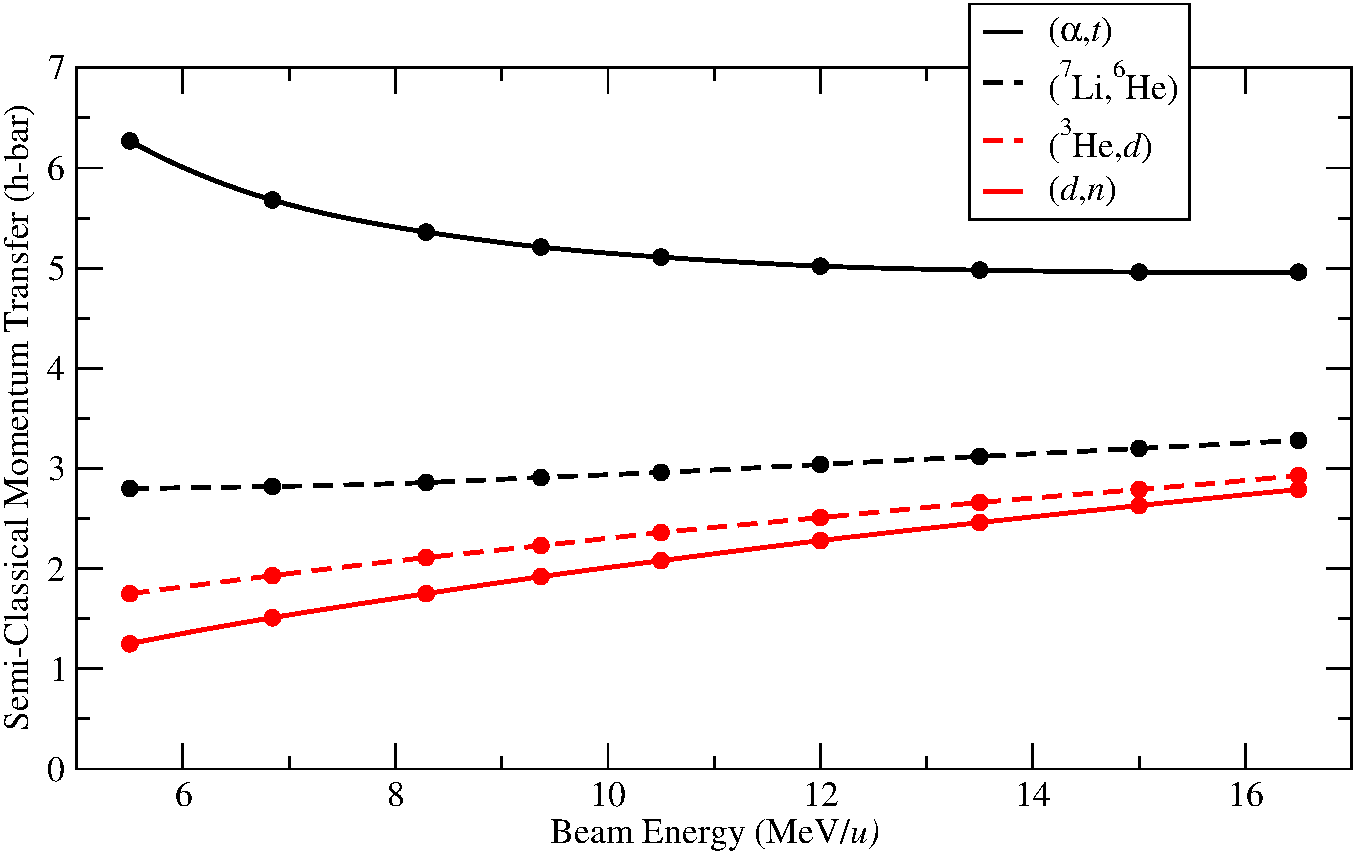
\includegraphics[width=0.9\columnwidth,height=0.4\textheight,keepaspectratio]{118Sn_l-matching}%
\caption[Semi-classical calculations of momentum-matching for proton-stripping reactions on $^{118}$Sn]{Semi-classical calculations of momentum-matching for proton-stripping reactions on $^{118}$Sn.  The calculated angular momentum transfer (in units of $\hbar$) is plotted as a function of beam energy.}%
\label{l_matching}%
\end{figure}

\begin{figure}%
\centering
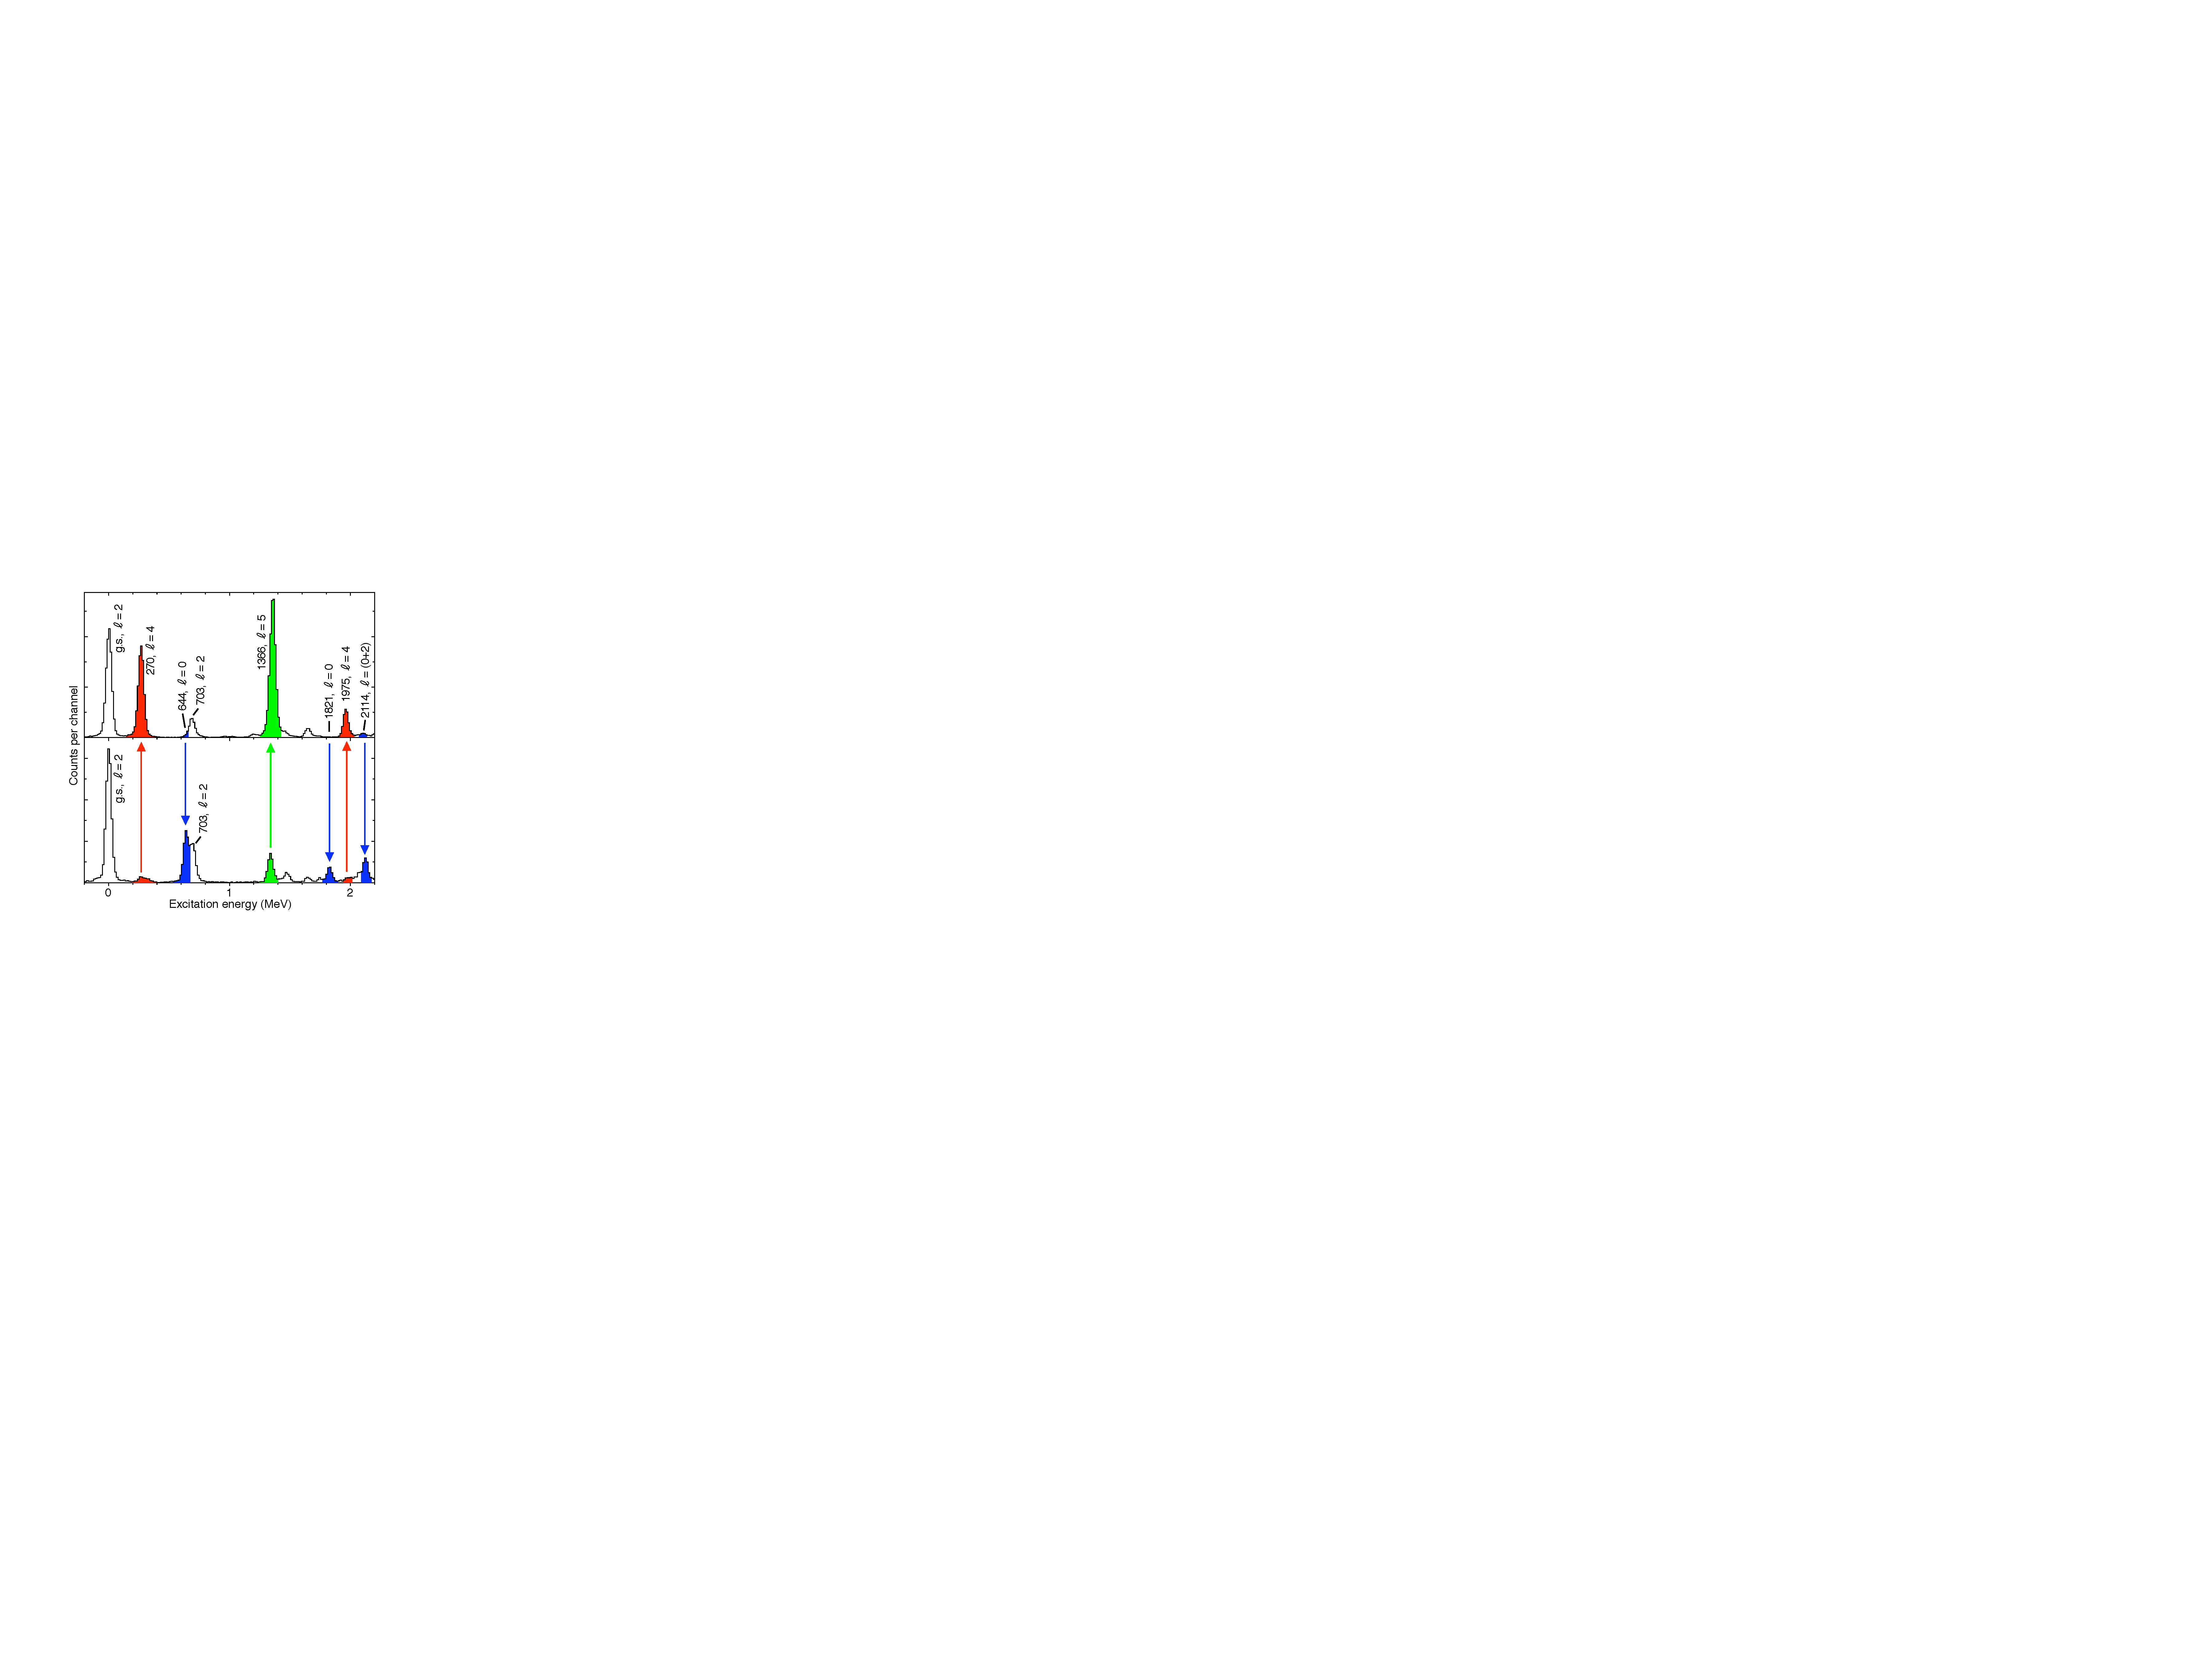
\includegraphics[width=\columnwidth,height=0.4\textheight,keepaspectratio]{matching_plot}%
\caption[Demonstration of momentum matching with two proton-stripping reaction on $^{118}$Sn]{Demonstration of momentum matching with two different proton-stripping reactions on $^{118}$Sn.  (Top) The $^{118}$Sn($\alpha$,$t$)$^{119}$Sb reaction, which has a large, negative $Q$-value of -14.7\,MeV, has enhanced yield to transitions corresponding to momentum transfers of $\ell=4$ and $\ell=5$. (Bottom) The yield to higher-spin states populated with the $^{118}$Sn($^3$He,$d$)$^{119}$Sb reaction is reduced and the low-spin states are enhanced.  Figure by B.~P.\ Kay from Ref.~\cite{Kay_2010PC}}%
\label{l_matching_spectra}%
\end{figure}

Continuing further with a naive picture of nuclear scattering, if the effects of the Coulomb field are neglected, the incoming plane-wave can be modeled as scattering from a hard sphere.  The Fraunh\"ofer diffraction equation
\begin{equation}
f(\theta)=\frac{ik}{4\pi}(1+\cos \theta)\int_S{e^{(i\vec{q}\cdot \vec{r})}dS}
\label{eq:1}
\end{equation}
gives the scattering amplitude as a function of angle and momentum transfer~\cite{Satchler_1990}.  Rewritten in terms of a differential cross section, this relationship becomes
\begin{equation}
\frac{d \sigma}{d \Omega}=k^2 r_0^4 \left[\frac{j_\ell(kr_0\theta)}{kr_0\theta}\right]^2
\label{eq:3}
\end{equation}
where $j_\ell(kr_0\theta)$ spherical Bessel function of order $\ell$.  
%Many nuclear properties have been studied by bombarding heavy nuclei with beams of light ions.  
This relationship shows that measuring the angular variations in the intensity of the energy levels provides additional useful information.  There is a direct relationship between the angular momentum $\ell$ transferred to the heavy recoil and the angular distribution of the ejected particle.  The resultant angular distribution is proportional to $j_\ell(kr_0\theta)$. Fig.~\ref{si_ang} shows an example of angular distributions from the $^{28}$Si($d$,$p$)$^{29}$Si reaction which exhibit an interference pattern comparable to Eq.~\ref{eq:3}.

\begin{figure}%
\centering
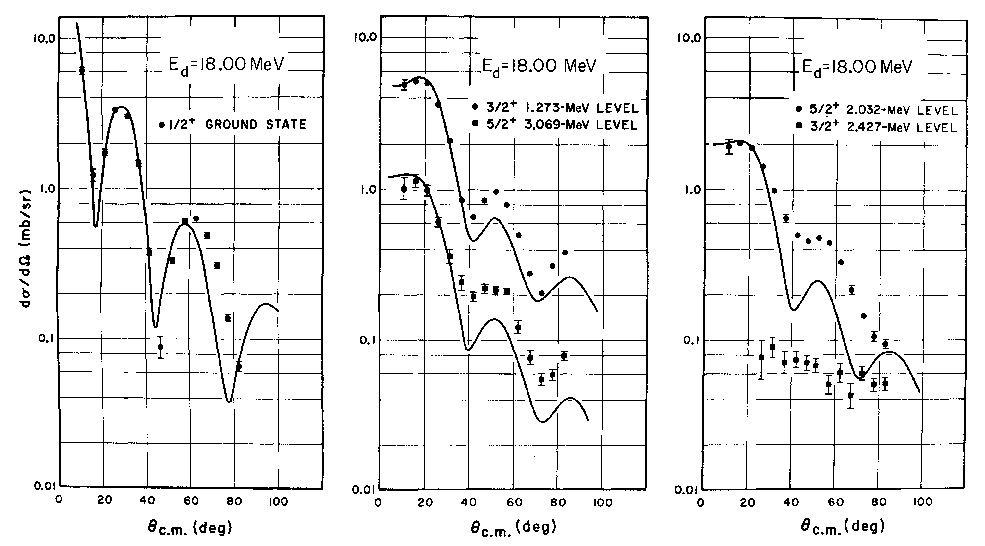
\includegraphics[width=\columnwidth]{Mermaz_fig_2}
\caption[Angular distributions from the $^{28}$Si($d$,$p$)$^{29}$Si reaction in normal kinematics]{Angular distributions from the $^{28}$Si($d$,$p$)$^{29}$Si reaction in normal kinematics.  Shown here are the angular distributions of four levels populated in the $^{28}$Si($d$,$p$)$^{29}$Si reaction at 9\,\AMeV{} with DWBA fits.  Figure from \citet[Fig.~1]{Mermaz_1971}.}
\label{si_ang}
\end{figure}

\section{Optical Model}
The phenomenological optical model was developed to improve upon the limitations of the plane wave theory of reactions.  The optical model characterizes the reaction by a potential which \textit{distorts} the incoming and outgoing plane waves.
\subsection{Nuclear Potentials}
%\subsubsection{Coloumb}
The optical model potential approximates the nuclear potential as
\begin{equation}
U(r)=-V f(r,r_0,a)-iW f(r,R^\prime,a^\prime)-iW_D g(r,r_0^\prime,a^\prime)
\label{eq:optical_im}
\end{equation}
where $V$ depths of the real parts of the Woods-Saxon potential, $W$ is the depth of the imaginary (absorption) part of the Woods-Saxon potential and $W_D$ is the strength surface-peaked imaginary potential.  The surface potential $g(r)$ is given by the derivative of the Woods-Saxon potential.
\begin{equation}
g(r,r_0^\prime,a^\prime)=4a\frac{d}{dr}f(r,r_0^\prime,a^\prime)
\label{eq:surface}
\end{equation}
In a similar fashion, the radial dependence of the spin-orbit term in Eq.~\ref{eq:woods_saxon} may be rewritten in terms of $g_\mathrm{SO}=r^{-1}(d/dr)f(r,r_\mathrm{SO},a_\mathrm{SO})$.  The exact depths of the real potentials are varied to reproduce the previously-known nucleon separation energy for a given nucleus.  The potential given in Eq.~\ref{eq:optical_im} includes imaginary terms in order to allow the removal of flux from the elastic scattering channel, \textit{i.e.}, for inelastic scattering.
%\subsection{Partial Wave Analysis}
\subsection{Distorted Wave Born Approximation}
\label{dwba}
Except for a number of special cases, the solutions to the Schr\"odinger equation for the optical model potential do not have a closed form and require computational solutions~\cite{Glendenning_2004}.  Calculating transition amplitudes for direct reactions in this way is called the distorted-wave Born approximation (DWBA).  By comparing the measured shape of the angular distributions from an experiment to DWBA calculations, the angular momentum transfer $l$ can be determined and the degree to which the states are accurately described as a single-particle state.  This provides a clear way of assigning the spin to the states populated in the heavy recoil.  The relationship between the measured angular distribution  and the calculated angular distribution is given by

\begin{equation}
\left(\frac{d\sigma}{d\Omega}\right)_\textrm{meas}=S\left(\frac{d\sigma}{d\Omega}\right)_\textrm{DWBA}
\label{eq:}
\end{equation}
where $S$ is called the spectroscopic factor.  For a state perfectly describe as a nucleon orbiting an closed core, that is, a single-particle state, the spectroscopic factor is identically equal to one.  The spectroscopic factor provides a measure of the overlap between the final state and the initial state plus an added nucleon.  Fig.~\ref{dwba_ediff} shows an example of calculations using the finite-range DWBA code PTOLEMY~\cite{Macfarlane_1978} using optical model parameters from Chapt.~\ref{exp} for the $^{28}$Si($d$,$p$) reaction at a variety of bombarding energies.

\begin{figure}%
\centering
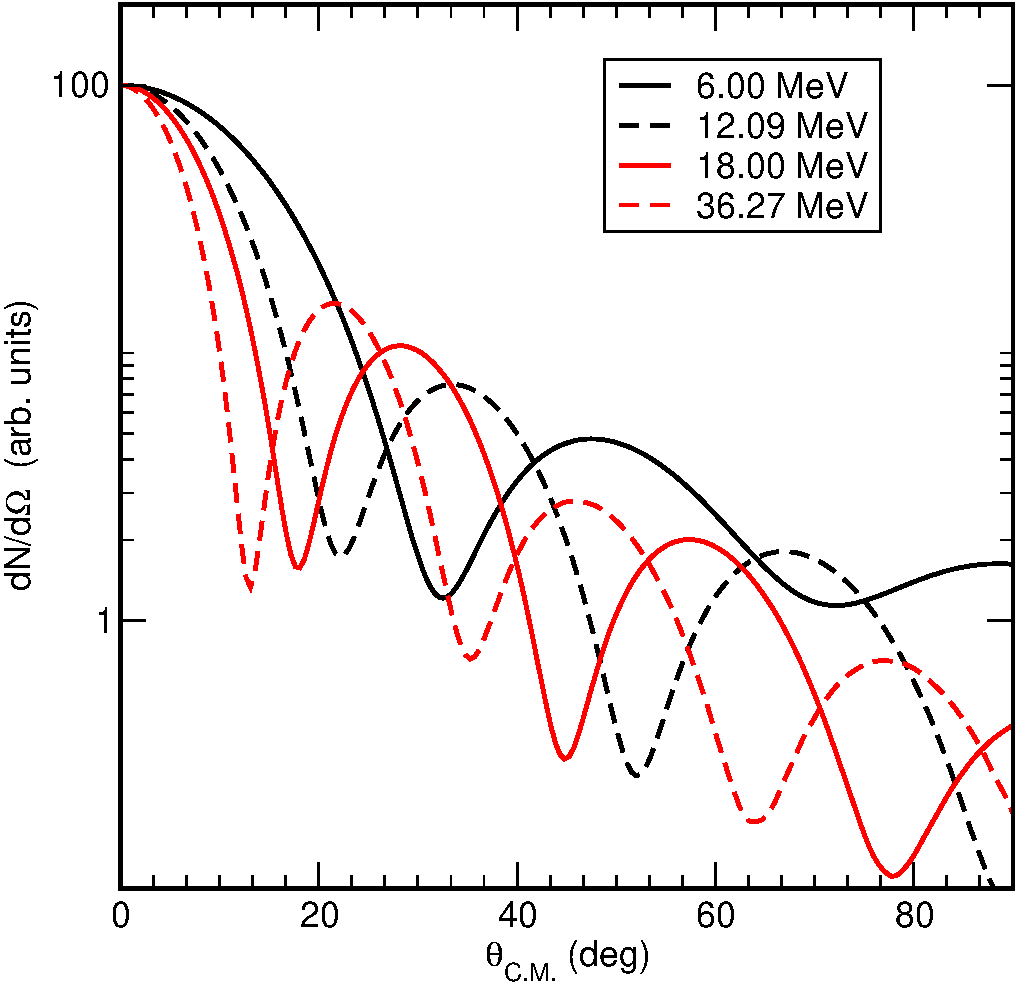
\includegraphics[width=\columnwidth,height=0.4\textheight,keepaspectratio]{angdist_curves_ediff}%
\caption[DWBA calculations for the $^{28}$Si($d$,$p$) reaction at four different bombarding energies]{DWBA calculations for the $^{28}$Si($d$,$p$) reaction at four different bombarding energies.  The calculations were carried out for the $\ell_n=0$ transitions to the $^{29}$Si ground state using the code PTOLEMY.  The cross sections have been normalized to $dN/d\Omega=100$ at $\theta_\mathrm{cm}$.}%
\label{dwba_ediff}%
\end{figure}

\section{Conclusion}
With few exceptions, most stable-beam stable-target combinations have been studied in terms of nucleon transfer reactions.  In order to measure the properties of nuclei further away from stability, it is necessary to utilize either radioactive beams or radioactive targets.  In principle, this technique would be useful to study exotic nuclei.  In terms of the $r$-process, it would be particularly useful to study neutron-rich nuclei with the ($d$,$p$) reaction which deposits a neutron on the target nucleus.  However, the nuclei of interest are so unstable that they are unsuitable for making targets.  Until recently, this limitation has made transfer reactions inapplicable to the study of exotic nuclei.  With the arrival of rare isotope beam capabilities at nuclear accelerator facilities, exotic nuclei can now be studied with this powerful technique.

The worldwide development of radioactive ion beam facilities is allowing for a new generation of nuclear reactions to be studied.  Reactions utilizing such exotic beams are permitting measurements of nuclear properties further away from stability than previously possible.  With radioactive beams, however, the kinematics of the measurement must be inverted, with a heavy-ion beam bombarding a light-ion target.  The basic form of the reactions being studied is the same (nucleon stripping or knock-out), but the reaction kinematics are changed in a way which presents new measurement difficulties.

%\section{Observables}
%
%\subsection{Angular Distribution}
%
%\subsection{Cross Section}
%\subsubsection{Spectroscopic Factor}
%
%Overlap between initial and final states.  Comparison between theory and experiment.  A measure of the single particle strength of the orbit. %\cite{Jiang_2009}
%\subsubsection{Selectivity}
%preferentially populates states with single-particle nature.~\cite{Wuosmaa_2005PRC,Wuosmaa_2008}